Consider the following command with GNU-style options shown:

\begin{Shaded}
\begin{Highlighting}[]
\ExtensionTok{yt{-}dlp} \AttributeTok{{-}{-}restrict{-}filenames} \AttributeTok{{-}{-}windows{-}filenames} \AttributeTok{{-}{-}mtime} \AttributeTok{{-}{-}write{-}auto{-}subs} \AttributeTok{{-}{-}embed{-}subs} \AttributeTok{{-}{-}embed{-}metadata} \AttributeTok{{-}{-}embed{-}chapters} \AttributeTok{{-}{-}xattrs} \AttributeTok{{-}{-}no{-}remove{-}chapters} 
\end{Highlighting}
\end{Shaded}

Assuming you have the program
\href{https://github.com/yt-dlp/yt-dlp}{yt-dlp} installed, that
invocation with the URL of a video at the end will grab the video,
restrict the resulting filename from having incompatible characters,
structure the filename to Windows conventions, set the file-modification
time to the last modified header's time, write and embed automatically
generated subtitles if they're available, embed metadata, embed
chapters, and write metadata to extended filesystem attributes if it can
do so in your operating system. Some of those are \emph{default}
behaviors of the program but it does help me to have it explicitly
written out for when I need to start modifying snippets. Sometimes I
can't recall the logic of a snippet and I can find things in a manual
page faster that way.

Now consider the following command snippet:

\begin{Shaded}
\begin{Highlighting}[]
\ExtensionTok{yt{-}dlp} \AttributeTok{{-}{-}restrict{-}filenames} \AttributeTok{{-}{-}windows{-}filenames} \AttributeTok{{-}{-}mtime} \AttributeTok{{-}{-}write{-}auto{-}subs} \AttributeTok{{-}{-}embed{-}subs} \AttributeTok{{-}{-}embed{-}metadata} \AttributeTok{{-}{-}embed{-}chapters} \AttributeTok{{-}{-}xattrs} \AttributeTok{{-}{-}no{-}remove{-}chapters} \StringTok{"https://archive.org/details/IBMPerso1987"}
\end{Highlighting}
\end{Shaded}

Assuming nothing went wrong that would download for you an episode of
the \emph{Computer Chronicles} related to the IBM PS/2. It is a program
hosted by Stewart Cheifet.

\begin{figure}
\centering
\pandocbounded{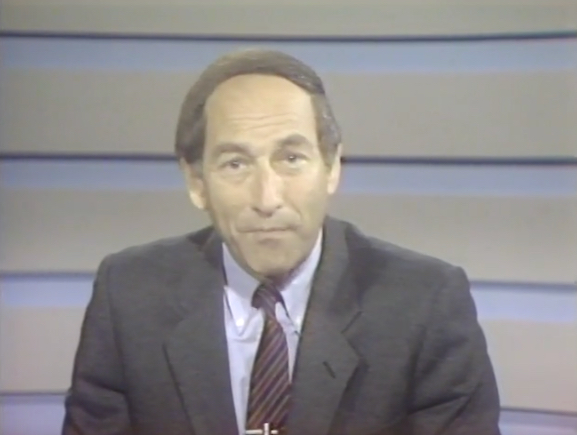
\includegraphics[keepaspectratio]{\%7B\%7Bsite.url\%7D\%7D/img/stewart-screenshot.jpg}}
\caption{A screen grab of the episode of Computer Chronicles referenced
above showing Stewart Cheifet during the Random Access segment talking
about Carnegie Mellon University.}
\end{figure}

Normally people think of peoples like yt-dlp for grabbing things solely
from YouTube. If you list its extractors you find that you can grab from
quite a few other places.

As things continue to fall apart around us, now would be a good time to
archive things more. Born digital content is ephemeral. Such things seem
to have better chances of long-term survival being transferred to film
at the rate changes in the legal environment are taking place.
